\documentclass{article}

% If you're new to LaTeX, here's some short tutorials:
% https://www.overleaf.com/learn/latex/Learn_LaTeX_in_30_minutes
% https://en.wikibooks.org/wiki/LaTeX/Basics

\def\rd{{\rm d}}
\def\ds{\displaystyle}

% Formatting
\usepackage[utf8]{inputenc}
\usepackage[margin=1in]{geometry}
\usepackage[titletoc,title]{appendix}

% Math
% https://www.overleaf.com/learn/latex/Mathematical_expressions
% https://en.wikibooks.org/wiki/LaTeX/Mathematics
\usepackage{amsmath,amsfonts,amssymb,mathtools}

% Images
% https://www.overleaf.com/learn/latex/Inserting_Images
% https://en.wikibooks.org/wiki/LaTeX/Floats,_Figures_and_Captions
\usepackage{graphicx,float}

% Tables
% https://www.overleaf.com/learn/latex/Tables
% https://en.wikibooks.org/wiki/LaTeX/Tables

% Algorithms
% https://www.overleaf.com/learn/latex/algorithms
% https://en.wikibooks.org/wiki/LaTeX/Algorithms
\usepackage[ruled,vlined]{algorithm2e}
\usepackage{algorithmic}

% Code syntax highlighting
% https://www.overleaf.com/learn/latex/Code_Highlighting_with_minted
\usepackage{minted}
\usemintedstyle{borland}

% References
% https://www.overleaf.com/learn/latex/Bibliography_management_in_LaTeX
% https://en.wikibooks.org/wiki/LaTeX/Bibliography_Management
\usepackage{biblatex}
\addbibresource{references.bib}

% Title content
\title{AMATH 482 Homework 2}
\author{Yiping Li}
\date{February 5, 2021}

\begin{document}

\maketitle

% Abstract
\begin{abstract}
    In this study, we are going to analyze a portion of two of the greatest rock and roll songs of all time: \textit{Sweet Child O' Mine} by Guns N' Roses and \textit{Comfortably Numb} by Pink Floyd. Our first task is to reproduce the music score for the guitar in the \textit{Sweet Child O' Mine} (GNR clip), and then we also are asked to isolate the music score for \textbf{bass} and \textbf{guitar} in the \textit{Comfortably Numb} (Floyd clip), one at the time.
\end{abstract}

% Introduction and Overview
\section{Introduction and Overview}
% Example Subsection
\subsection{Problem Setting}
Our task is reproducing the music score of each clip from a portion of the sound track. Notice that, each note has a corresponding frequency. Based on the table of music scale along with the frequency of each note in Hz, we are able to identify the note by analyzing the frequencies in the time domain. \\
~\\
However, the major obstacles of extracting the music scores are the existence of the overtone and overlaps of instruments. The overtone describes the phenomena that if we have a note produces 100 Hz sounds as the fundamental frequency, it will also produces an integer multiple of the fundamental frequency (n*100 Hz) because of the constructive interference. \\
~\\
In the GNR clip, the only playing instruments is guitar, therefore we only need to solve the problem of overtone. In the Floyd clip, both guitar and bass are playing, therefore we need to remove overtones and isolate them.

% Example Subsubsection
\subsection{Data Format}
Both clips are given by \textbf{.m4a} files. In the \textbf{GNR} clip, we are given a 14 seconds clips, which is loaded as a vector with 659,122 doubles into the MATLAB. In the \textbf{Floyd} clip, we are given a 60 seconds clips, which loaded as a vector with 2,635,921 doubles into the MATLAB.


%  Theoretical Background
\section{Theoretical Background}
Since we have discussed the Fast Fourier Transform (FFT) in the last study, we will skip it in this study. \\
~\\
The mechanism behind Gabor Transform is that we zoom in a specific moment at the time domain, which in other words, we apply a window function (filter) to focus on a specific time. There are many kinds of window functions, for this study, we used a Gaussian, which is defined as following
\begin{equation}
    g(t-\tau) = e^{-a(t-\tau)^2}.
\end{equation}
Here, $\tau$ is the horizontal shift of a Gaussian function. It also can be interpret as \textbf{the center of the window}. Moreover, $a$ is proportional to \textbf{the width of the window}, which is saying that larger $a$ indicates narrower width of the window.
~\\
It is worth to mention the balance between time information and frequency information. This is an unsolvable conflict. If we want to know more about time, we must scarifies the information about the frequency. Therefore, it is important to find an appropriate value for $a$ and $\tau$ to generate a clean graph.


% Algorithm Implementation and Development
\section{Algorithm Implementation and Development}
\subsection{Preparation}
In this section, we are initialize some fundamental variables for the time domain and the frequency domain.
\begin{algorithm}
\begin{algorithmic}
    \STATE{Importing data from \texttt{GNR.m4a}}
    \STATE{Define the size of the time domain (t)}
    \STATE{Define the size of the frequency domain (k)}
\end{algorithmic}
\caption{Preparation}
\end{algorithm}

\subsection{Finding the fundamental frequency range}
Again, the conflict between the time and the frequency is always there, therefore before we apply the window filter, looking at a specific moment, we can sacrifices the information in time to get a overall image of the frequency domain. \\
Thus, the first thing we do here is to check how does the frequency domain looks like by \texttt{fft}.

\begin{algorithm}
\begin{algorithmic}
    \STATE{Project the sound wave into the frequency domain}
    \STATE{Plot and interpret the graph}
\end{algorithmic}
\caption{Transforming to the frequency domain}
\end{algorithm}
\begin{figure}[h]
    \centerline{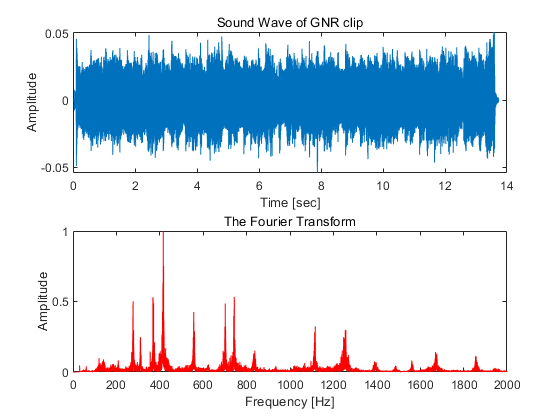
\includegraphics[width=3in]{overall_GNR.png}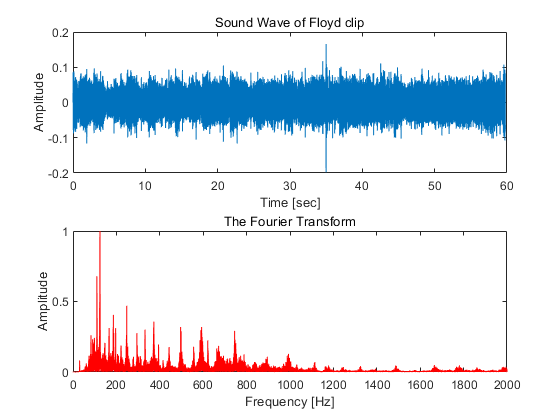
\includegraphics[width=3in]{overall_Floyd.png}}
    \caption{The overall view of sound wave in both the time and the frequency domain. GNR (left); Floyd (right)}
\end{figure}

Here, notice that in the GNR clip, guitar is the only instrument in this portion. Therefore, we should be able to observe the fundamental frequencies and their overtones in the frequency domain. In fact, let's look at the the first three pulses (with large amplitude) located at $k=290, 390, 410$. This pattern actually repeats. The first repeat is at where $k=570,790,810$, and the second repeat is at where $k=810,1100,1240$. Moreover, the frequency with the maximum amplitude is about 400 Hz. Therefore, we conclude that the fundamental frequency is around 300 Hz. \\
~\\
As for the Floyd clip, the situation is more complicated since it involves two instruments. However, the frequency with the maximum amplitude is around 150 Hz, and based on the research, bass produces sounds with frequency between 16-256 Hz. Therefore, we can assume that the fundamental frequencies are around 100 Hz.


\subsection{Applying the Gabor Transform}
Now, we are going to apply Gabor Transform with appropriate $a$ and $d\tau$. Notice that, we are not apply the filter at one specific moment, instead, we are moving the filter window along the time domain. Therefore, the parameter we need to determine is $d\tau$, the step of the window. For the GNR clip, we selected $a=2000$ and $d\tau=0.1$. As for the Floyd clip, we selected $a=2000$ and $d\tau=1$ due to the memory capacity of the device. \\
~\\

\begin{algorithm}
\begin{algorithmic}
    \STATE{Initialize parameter for Gabor Transform}
    \FOR{$i=0:d\tau:end$}
        \STATE{Define the Gauss filter centered at \texttt{t=i}}
        \STATE{Apply the filter to the sound wave, multiplying it by the filter}
        \STATE{Transform the signal into the frequency domain by \texttt{fft}}
        \STATE{Store the result}
    \ENDFOR
    \STATE{Plot the spectrogram by \texttt{pcolor}}
\end{algorithmic}
\caption{Applying the Gabor Transform}
\end{algorithm}
\begin{figure}[h]
    \centerline{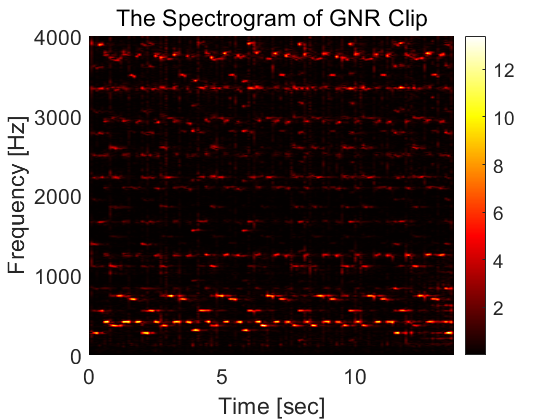
\includegraphics[width=3in]{spect_GNR.png}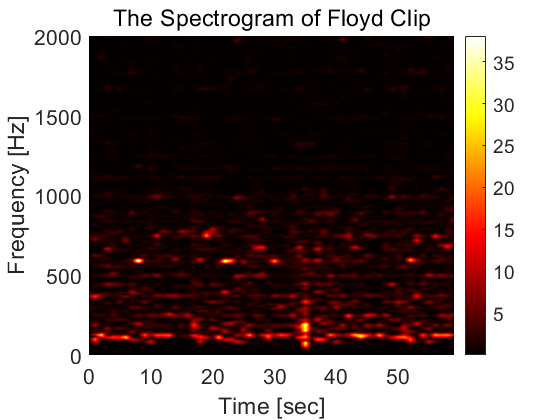
\includegraphics[width=3in]{spect_Floyd.png}}
    \caption{The spectrogram (Frequency vs. Time) of GNR clip (left) and Floyd clip (right).}
\end{figure}

\subsection{Extracting the Fundamental Frequencies}
Notice that the FFT will give us the information of all frequencies, including the overtones of the fundamental frequencies. To extract the fundamental frequencies, we only need to apply some filters on the frequency domain to emphasize on a specific frequency range. Based on the analysis we have done in 3.2, we have found the possible fundamental frequency range. Therefore, we are going to apply another filter on the frequency domain to focus on those specific ranges of frequency. Here, we used a Gauss, again. \\
~\\
For the GNR clip, we selected $a=0.000004$ and $k_c=300$. 
\begin{equation}
    gk_{fund} = e^{-0.000004(k-300)^2}
\end{equation}
As for the Floyd clip, we selected $a=0.000004$ and $k_c=200$ to extract the fundamental frequencies of bass.
\begin{equation}
    gk_{fund} = e^{-0.000004(k-100)^2}
\end{equation}
\begin{algorithm}
\begin{algorithmic}
    \STATE{Initialize parameter for Gabor Transform}
    \FOR{$i=0:d\tau:end$}
        \STATE{Define the Gauss filter centered at \texttt{t=i}}
        \STATE{Apply the filter to the sound wave, multiplying it by the filter}
        \STATE{Transform the signal into the frequency domain by \texttt{fft}}
        \STATE{\textbf{Apply the Gauss filter on the frequency domain.}}
        \STATE{Store the result}
    \ENDFOR
    \STATE{Plot the spectrogram by \texttt{pcolor}}
    \STATE{Label the note}
\end{algorithmic}
\caption{Extracting the Fundamental Frequencies}
\end{algorithm}
\begin{figure}[h]
    \centerline{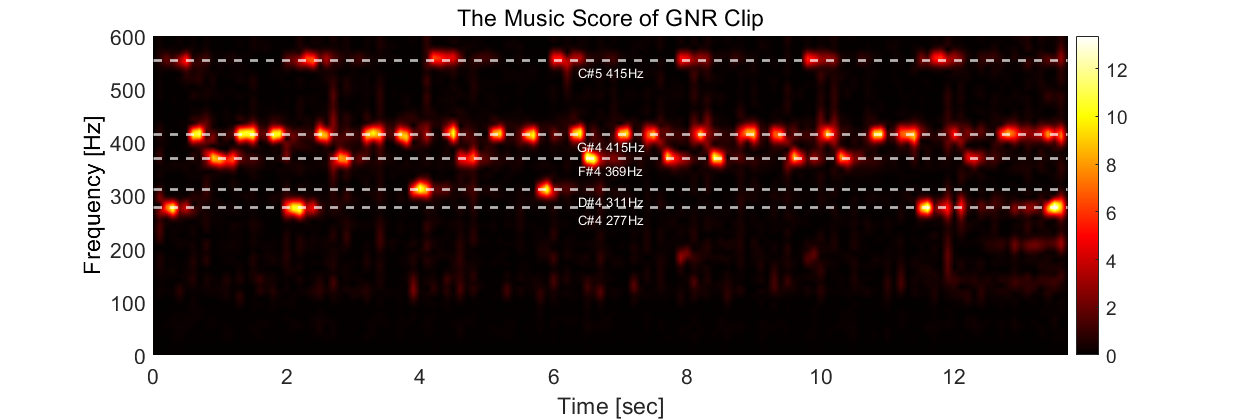
\includegraphics[width=6in]{music_score_GNR.png}}
    \caption{The spectrogram of the GNR clip after applying a Gauss filter on the frequency domain}
\end{figure}\\
Since we have filter out the overtones, we have a clear graph with time in the x-axis and frequency in the y-axis. Based on that, we can restore the music score of guitar in the GNR clip, which is shown in the Figure 3.\\
\begin{figure}[h]
    \centerline{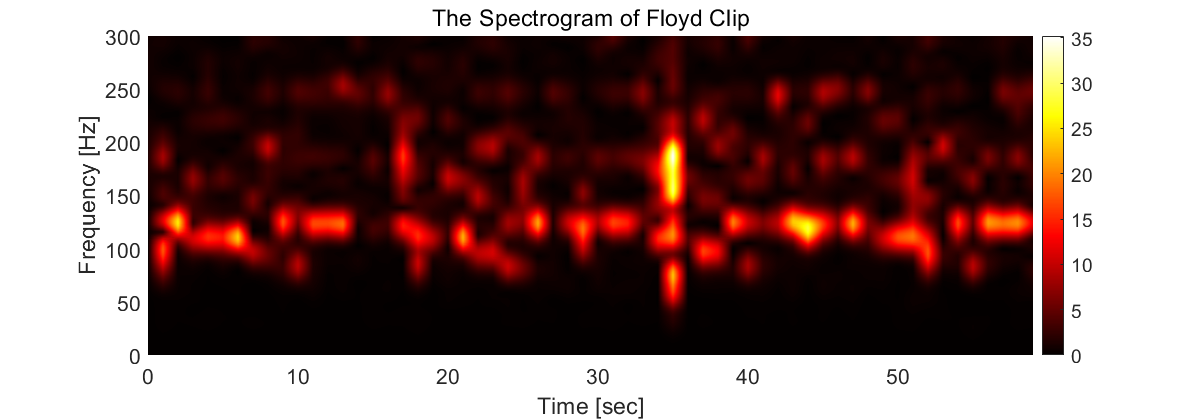
\includegraphics[width=6in]{music_score_Floyd_1.png}}
    \caption{The spectrogram of the Floyd clip after applying a Gauss filter on the frequency domain}
\end{figure}
\newpage
Notice that, we have a really blurry graph here for the Floyd clip. We predict that it might be caused undersampling, as for the result of large window step ($d\tau=1$). Another reason might be the size of the filter applied on the frequency domain. Since the sound wave is more chaotic, we decided to apply another filter on the frequency domain.

\subsection{Applying an Additional Filter on the Frequency Domain}
As previously mentioned, we decided to have another filter to clean up the graph. This time, we want to apply the filter around the frequency around 150 Hz with the maximum intensity. Again, a Gauss filter is used. Most steps here are the same, the additional steps are bolded.
~\\
For this additional filter, we selected $a=0.04$. 
\begin{equation}
    gk_{max} = e^{-0.004(k-k_max)^2}
\end{equation}

\begin{algorithm}
\begin{algorithmic}
    \STATE{Initialize parameter for Gabor Transform}
    \FOR{$i=0:d\tau:end$}
        \STATE{Define the Gauss filter centered at \texttt{t=i}}
        \STATE{Apply the filter to the sound wave, multiplying it by the filter}
        \STATE{Transform the signal into the frequency domain by \texttt{fft}}
        \STATE{Apply the Gauss filter on the frequency domain.}
        \STATE{\textbf{Find the frequency with the maximum intensity by \texttt{max}}}
        \STATE{\textbf{Apply another Gauss filter on the frequency with the maximum intensity}}
        \STATE{Store the result}
    \ENDFOR
    \STATE{Plot the spectrogram by \texttt{pcolor}}
    \STATE{Label the note}
\end{algorithmic}
\caption{Applying an Additional Filter on the Frequency Domain}
\end{algorithm}
\begin{figure}[h]
    \centerline{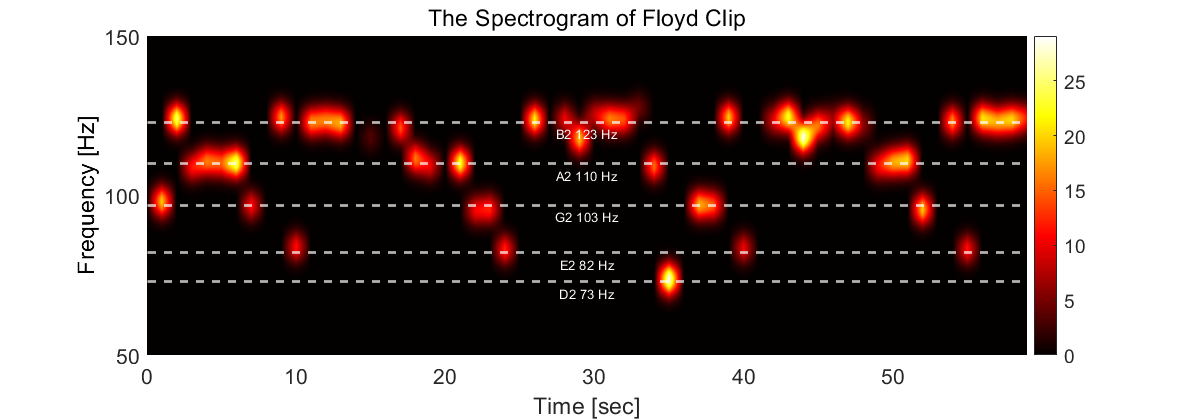
\includegraphics[width=6in]{music_score_Floyd_2.png}}
    \caption{The spectrogram of the Floyd clip after applying an additional Gauss filter around the frequency$_{max}$}
\end{figure}
Applying an additional Gauss filter indeed gives us a cleaner spectrogram, which allowed us to mark the note. 
\newpage
\subsection{Extracting the Frequencies Produced by a Guitar}
Since a guitar produces higher frequency than a bass, which means that the overtones of the sound produced by a bass are mixed with the frequencies produced by a guitar. Therefore we can't simply extracting the frequencies in certain range, instead, we are going to remove the overtone frequencies. \\
First, we need to find the fundamental frequency produced by a bass, which can be done by tracking the frequency with the maximum intensity. If it is below 200 Hz, we can assume that is is produced by a bass. \\
Second, we used a "inverted" Gauss filter, which defined as the following
\begin{equation}
    gk_{remove} = (1 - e^{-0.0004(k-nk_{fundamental})^2}
\end{equation}
This inverted Gauss filter will set the intensity at the center frequency to 0, and reduce the intensity around the center frequency. Similar portions are emitted. We will apply the filter to the integer multiples of the fundamental frequency, \\
Lastly, we apply the filter we used in section 3.5 to emphasize on the frequency with the maximum intensity at that moment. \\

\begin{algorithm}
\begin{algorithmic}
    \FOR{$i=0:d\tau:end$}
        \STATE{...}
        \STATE{Transform the signal into the frequency domain by \texttt{fft}}
        \STATE{Find the frequency with the maximum intensity}
        \IF{$k_{max} < 200$}
            \FOR{$i=1:20$}
                \STATE{Apply the inverted Gauss filter at $k_{fund} = k_{max}$}
            \ENDFOR
        \ENDIF
        \STATE{Set the intensity of the frequency below 200 Hz to 0}
        \STATE{Find the frequency with the maximum intensity}
        \STATE{Apply the Gauss filter (in 3.5) on the frequency with the maximum intensity}
        \STATE{Store the result}
    \ENDFOR
    \STATE{Plot the spectrogram by \texttt{pcolor}}
    \STATE{Label the note}
\end{algorithmic}
\caption{Extracting the Frequencies Produced by a Guitar}
\end{algorithm}
\begin{figure}[h]
    \centerline{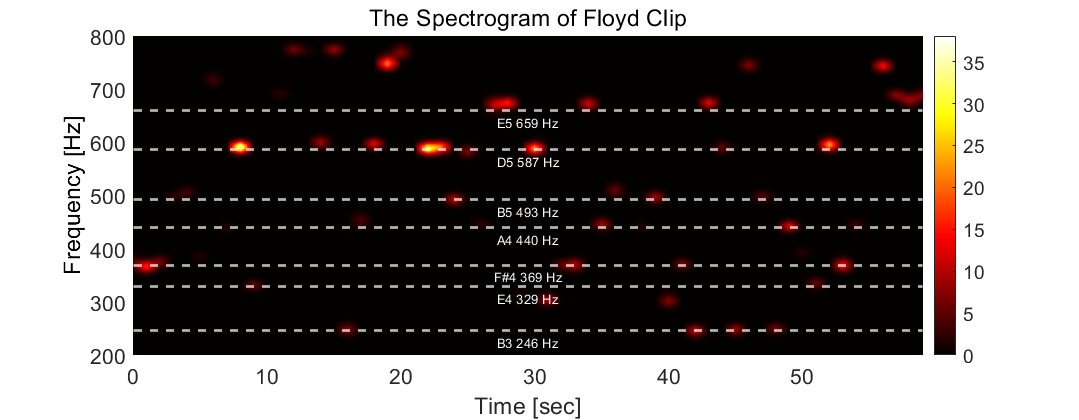
\includegraphics[width=6in]{music_score_Floyd_3.png}}
    \caption{The spectrogram of the Floyd clip after extracting the frequencies produced by a guitar}
\end{figure}


\newpage
\section{Computational Result}
In the study, we reproduced the music score of guitar from a portion of \textit{Sweet Child O’ Mine}. (Figure 7) \\
\begin{figure}[h]
    \centerline{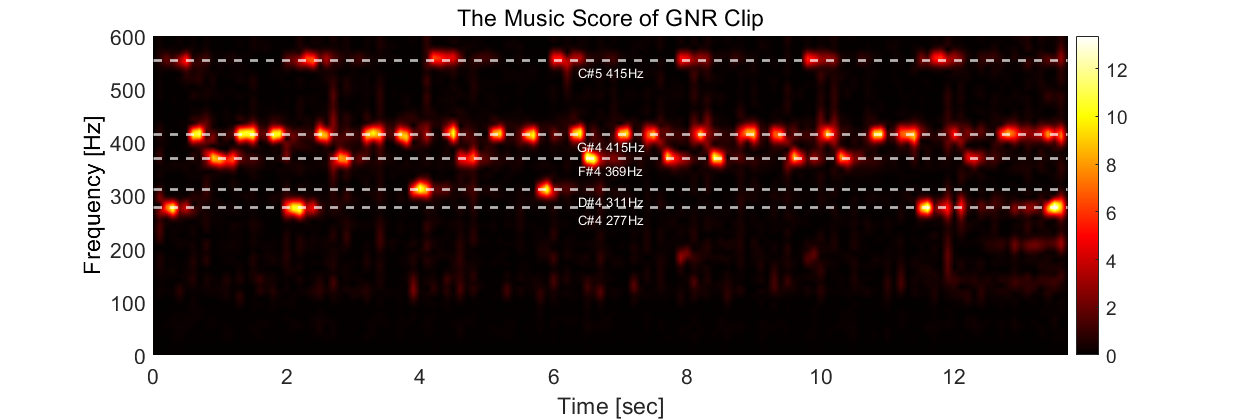
\includegraphics[width=6in]{music_score_GNR.png}}
    \caption{The music score of guitar in GNR clip (problem 1)}
\end{figure}\\
We also reproduced  music score of bass from a portion of \textit{Comfortable Numb}. (Figure 8) \\
\begin{figure}[h]
    \centerline{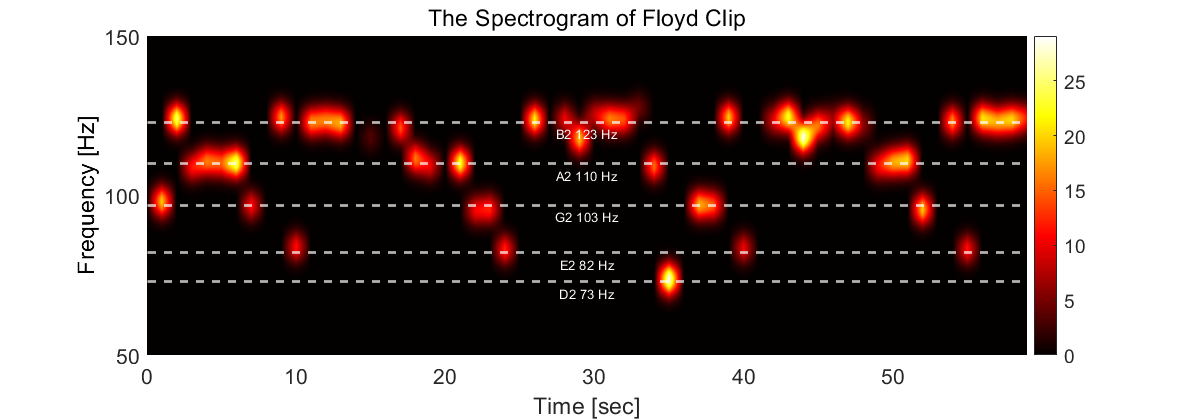
\includegraphics[width=6in]{music_score_Floyd_2.png}}
    \caption{The music score of bass in Floyd clip (problem 2)}
\end{figure}\\
Lastly, we reproduced  music score of guitar from a portion of \textit{Comfortable Numb}. (Figure 9)\\
\begin{figure}[h]
    \centerline{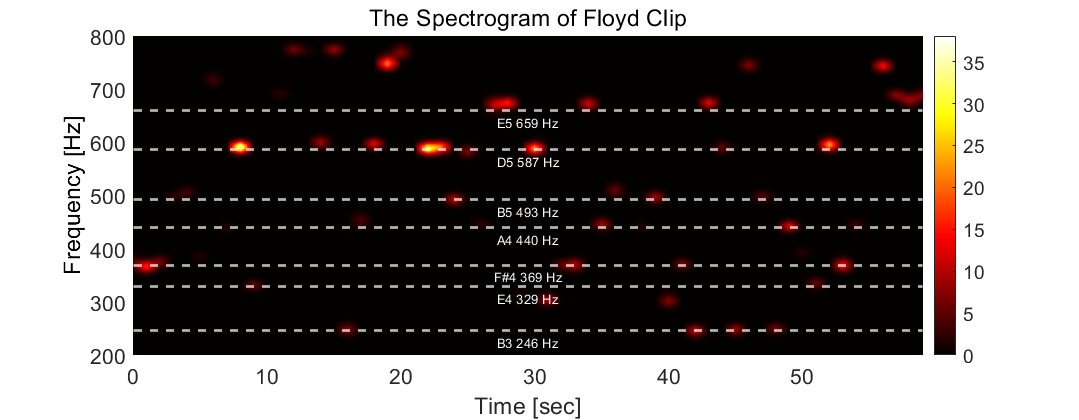
\includegraphics[width=6in]{music_score_Floyd_3.png}}
    \caption{The music score of guitar in Floyd clip (problem 3)}
\end{figure}\\

\newpage
\section{Summary and Conclusion}
In the study, we used the Fourier Transform to project sound wave to the frequency domain from time domain. Based on the graph, we are able to guess the fundamental frequencies produced by bass or guitar in the clips. \\
Next, applying a Gauss filter on time domain along the x-axis, we used the Gabor Transform to produce a spectrogram, which has time in x-axis and frequency in y-axis. It is important because we are able to obtain the information in both the frequency domain and the time domain, which is not possible for normal Fourier Transform. \\
Since the spectrogram is not clean, we applied another Gauss filter on the frequency domain to focus on the frequency in certain range. \\
To remove the overtones of the bass, we implemented an inverted Gauss filter, which is able to emit the frequencies around a given frequency. \\
It is worth to mention that the parameters of the filter were determined by several trails, we are not sure that those parameters are the most appropriate ones, especially for the inverted Gauss filter. Therefore, in the future study, more trails should be done to determine the parameters pf the inverted Gauss filter.
\newpage
% Appendices
\begin{appendices}

% MATLAB Functions
\section{MATLAB Functions}
\begin{itemize}
    \item \texttt{[M, I] = max(Sgn)} returns the linear indices of the 
    maximum values in vector \texttt{Sgn}
    \item \texttt{pcolor(X, Y, C)} where X and Y are vectors or matrices, makes a
    pseudo color plot on the grid defined by X and Y.  
\end{itemize}

% MATLAB Codes
\newpage
\section{MATLAB Code}

\begin{verbatim}
%% Clean workspace
%% Part 1 - GNR - guitar
clear all; close all; clc;

% load sound data
[S, Fs] = audioread('GNR.m4a');
% p8 = audioplayer(S,Fs); playblocking(p8); % play the sound track

% setup parameters
n = length(S);
t = (1:n) / Fs;
L = n / Fs;
k = (1/L)*[0:n/2-1 -n/2:-1]; ks = fftshift(k);


% vitualize the data
figure(1)
S = S'; St = fft(S);  
subplot(2, 1, 1);
plot(t, S);
xlabel('Time [sec]');
ylabel('Amplitude');
title('Sound Wave of GNR clip');

subplot(2, 1, 2);
plot(ks, abs(fftshift(St))/max(abs(St)), 'r');
set(gca, 'XLim', [0 2000]);
xlabel('Frequency [Hz]');
ylabel('Amplitude');
title('The Fourier Transform');

%% Apply Gabor filter

% parameters for the filter (window)
a = 2000;
tau = 0:0.1:L;

mm = 0;
mi = 0;
for j = 1:length(tau)   
    g = exp(-a*(t - tau(j)).^2); % Window function   
    Sg = g.*S;   
    Sgt = fft(Sg);
    
    [M, I] = max(Sgt); % find the frequency with the maximum intensity
    Sgt = Sgt.*exp(-0.000004*(k-300).^2); % apply the filter around that frequency
    
    Sgt_notes(:,j) = abs(k(I)/2*pi); % record the maximum frequency
    Sgt_spec(:,j) = fftshift(abs(Sgt)); % We don't want to scale it
end
%% Ploting
clc; close all;
figure(2)
pcolor(tau,ks, Sgt_spec)
shading interp
set(gca,'ylim',[0 600],'Fontsize',16)
colormap(hot)
colorbar
xlabel('Time [sec]'), ylabel('Frequency [Hz]', 'Color', 'black')
title('The Music Score of GNR Clip');

hold on;
y1 = yline(277,'--','C#4 277Hz', 'LineWidth', 2, 'Color','white');
y1.LabelVerticalAlignment = 'bottom';
y1.LabelHorizontalAlignment = 'center';

y2 = yline(311,'--','D#4 311Hz', 'LineWidth', 2, 'Color', 'white');
y2.LabelVerticalAlignment = 'bottom';
y2.LabelHorizontalAlignment = 'center';

y3 = yline(369,'--','F#4 369Hz', 'LineWidth', 2, 'Color', 'white');
y3.LabelVerticalAlignment = 'bottom';
y3.LabelHorizontalAlignment = 'center';

y4 = yline(415,'--','G#4 415Hz', 'LineWidth', 2, 'Color', 'white');
y4.LabelVerticalAlignment = 'bottom';
y4.LabelHorizontalAlignment = 'center';

y5 = yline(554,'--','C#5 415Hz', 'LineWidth', 2, 'Color', 'white');
y5.LabelVerticalAlignment = 'bottom';
y5.LabelHorizontalAlignment = 'center';
% figure(3)
% plot(tau, Sgt_notes, 'o')

%% Part 1 - Floyd - bass & guitar
clear all; close all; clc;

% load sound data
[S, Fs] = audioread('Floyd.m4a');
% p8 = audioplayer(S,Fs); playblocking(p8); % play the sound track

S = S(1: length(S)-1);
% setup parameters
n = length(S);
t = (1:n) / Fs;
L = n / Fs;
k = (1/L)*[0:n/2-1 -n/2:-1]; ks = fftshift(k);


% vitualize the data
figure(1)
S = S'; St = fft(S);  
subplot(2, 1, 1);
plot(t, S);
xlabel('Time [sec]');
ylabel('Amplitude');
title('Sound Wave of Floyd clip');

subplot(2, 1, 2);
plot(ks, abs(fftshift(St))/max(abs(St)), 'r');
set(gca, 'XLim', [0 2000]);
xlabel('Frequency [Hz]');
ylabel('Amplitude');
title('The Fourier Transform');

%% Apply Gabor filter
close all;
% parameters for the filter (window)
a = 2000;
tau = 0:1:L;

for j = 1:length(tau)
    g = exp(-a*(t - tau(j)).^2); % Window function   
    Sg = g.*S;   
    Sgt = fft(Sg);
    
    % subplot(2, 1, 1);
    % plot(ks, abs(fftshift(Sgt))/max(abs(Sgt)), 'r');

    
    [M, I] = max(Sgt); % find the frequency with the maximum intensity
    
    % if the frequency with the maximum intensity is lower than 200Hz
    if 0 < k(I) && k(I) <= 200
        freq = k(I);
        % bass was played
        for i = 1:50 % remove overtune
            Sgt = Sgt.* (1-exp(-0.0004*(k-freq*i).^2)); % apply the filter around that frequency
        end
    end
    
    % subplot(2, 1, 2);

    % plot(ks, abs(fftshift(Sgt))/max(abs(Sgt)), 'r');
        
    Sgt = Sgt.*(1-exp(-0.00004*(k-90).^2)); % remove frequencies around 90Hz (bass)
    Sgt(length(Sgt)/2:length(Sgt)) = 0; % remove negative requencies

    [M, I] = max(Sgt); % find the frequency with the maximum intensity
    % k(I)
    Sgt = Sgt.*exp(-0.004*(k-k(I)).^2); % apply the filter around the frequency with maximum intensity

    % Sgt_notes(:,j) = abs(k(I)/2*pi); % record the maximum frequency
    Sgt_spec(:,j) = fftshift(abs(Sgt)); % We don't want to scale it
end
%% 
close all;
figure(2)
pcolor(tau,ks, Sgt_spec)
shading interp
set(gca,'ylim',[200 800],'Fontsize',16)
colormap(hot)
colorbar
xlabel('Time [sec]'), ylabel('Frequency [Hz]', 'Color', 'black')
title('The Spectrogram of Floyd Clip');

hold on;
y1 = yline(369,'--','F#4 369 Hz', 'LineWidth', 2, 'Color','white');
y1.LabelVerticalAlignment = 'bottom';
y1.LabelHorizontalAlignment = 'center';

y2 = yline(246,'--','B3 246 Hz', 'LineWidth', 2, 'Color', 'white');
y2.LabelVerticalAlignment = 'bottom';
y2.LabelHorizontalAlignment = 'center'; 

y3 = yline(587,'--','D5 587 Hz', 'LineWidth', 2, 'Color', 'white');
y3.LabelVerticalAlignment = 'bottom';
y3.LabelHorizontalAlignment = 'center';

y4 = yline(493,'--','B5 493 Hz', 'LineWidth', 2, 'Color', 'white');
y4.LabelVerticalAlignment = 'bottom';
y4.LabelHorizontalAlignment = 'center';

y5 = yline(440,'--','A4 440 Hz', 'LineWidth', 2, 'Color', 'white');
y5.LabelVerticalAlignment = 'bottom';
y5.LabelHorizontalAlignment = 'center';

y6 = yline(659,'--','E5 659 Hz', 'LineWidth', 2, 'Color', 'white');
y6.LabelVerticalAlignment = 'bottom';
y6.LabelHorizontalAlignment = 'center';

y7 = yline(329,'--','E4 329 Hz', 'LineWidth', 2, 'Color', 'white');
y7.LabelVerticalAlignment = 'bottom';
y7.LabelHorizontalAlignment = 'center';

% yticks([-1 -0.8 -0.2 0 0.2 0.8 1])
% ticklabels({'-3\pi','-2\pi','-\pi','0','\pi','2\pi','3\pi'})

% figure(3)
% plot(tau, Sgt_notes, 'o')
\end{verbatim}


\end{appendices}

\end{document}
